\chapter*{Appendix}
\addcontentsline{toc}{chapter}{Appendices}

\begin{figure}[h]
\caption{Nunjucks File Structure}
  \label{fig:structure}
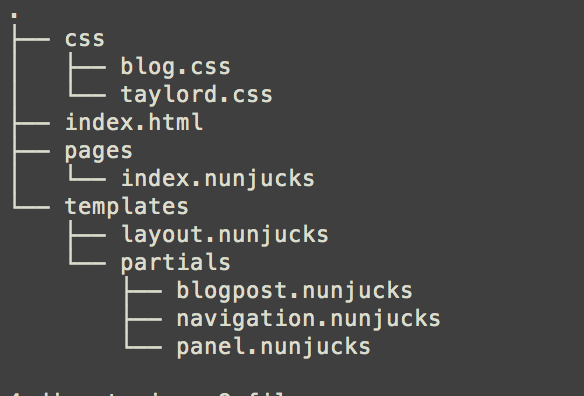
\includegraphics{../public/images/fileStructure}
\centering
\end{figure}

\begin{figure}[h]
\caption{12 grid layout with the 960 grid}
  \label{fig:grid}
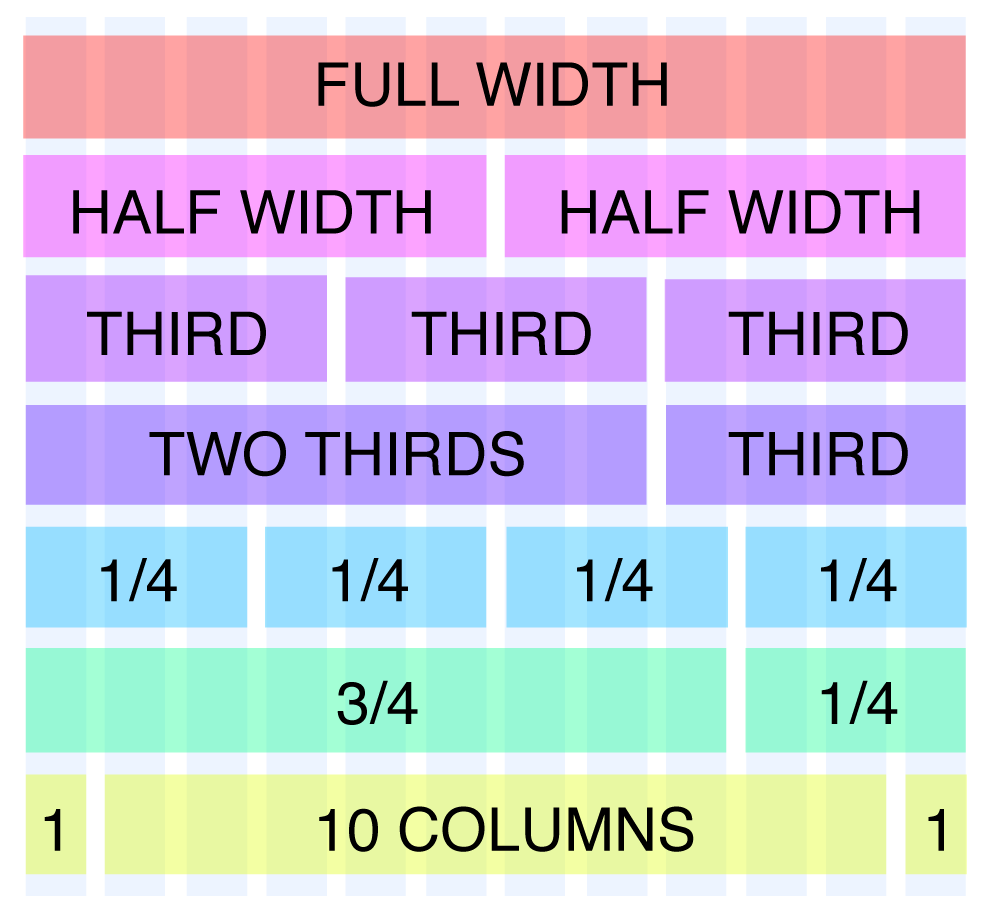
\includegraphics[scale=0.4]{../public/images/960-12-col-grid}
\centering
\end{figure}

\begin{figure}[h]
\caption{Chrome Developer Tools}
  \label{fig:tools}
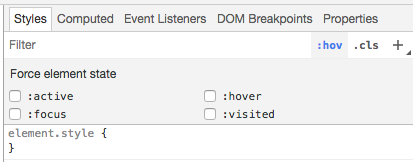
\includegraphics{../public/images/tools}
\centering
\end{figure}

%
%\begin{figure}
%\centering
%\includegraphics[width=8cm]{images/12}
%\caption{A searchlight beam model of Jupiter's decametric radio emissions \citep{imai-08}}
%\label{fig:decametric_emissions_searchlight}
%\end{figure}
%%
%
%%
%\begin{figure}
%\centering
%\includegraphics[width=8cm]{images/13}
%\caption{Io Flux Tube and the Plasma Torus \citep{lang-10}}
%\label{fig:io_flux_tube_plasma_torus}
%\end{figure}
%%
%
%%
%\begin{figure}	
%	\centering
%	\begin{subfigure}[t]{8cm}
%		\centering
%		\includegraphics[width=8cm]{images/14}
%		\caption{21 MHz Shortwave Loop Antenna Radio Telescope Design \citep{greef-12}}
%		\label{fig:loop_antenna_design_a}		
%	\end{subfigure}
%	\quad
%	\begin{subfigure}[t]{5cm}
%		\centering
%		\includegraphics[width=5cm]{images/16}
%		\caption{21 MHz Shortwave Loop Antenna Radio Telescope Design \citep{greef-12}}
%		\label{fig:loop_antenna_design_b}
%	\end{subfigure}
%	\quad
%	\begin{subfigure}[t]{5cm}
%		\centering
%		\includegraphics[width=5cm]{images/15}
%		\caption{21 MHz Shortwave Loop Antenna Radio Telescope Design \citep{greef-12}}
%		\label{fig:loop_antenna_design_c}
%	\end{subfigure}
%	\caption{21MHz Shortwave Loop Design}
%	\label{fig:loop_antenna_design}
%\end{figure}
%
%

\newpage
\begin{table}[!ht]
\centering
\caption{Framework features}
\label{features}
\begin{tabular}{llll}
 & Bootstrap & Foundation & Skeleton \\
Alerts & Yes & Yes & No \\
Accordion & Yes & Yes & No \\
Badges & No & Yes & No \\
Breadcrumbs & Yes & Yes & No \\
Buttons & Yes & Yes & Yes \\
Carousel & Yes & Yes & No \\
Dropdown & Yes & Yes & No \\
Forms & Yes & Yes & Yes \\
Form Validation & Yes & Yes & No \\
Grid & Yes & Yes & Yes \\
Icons & No & Yes & No \\
Labels & Yes & Yes & No \\
Lists & Yes & Yes & Yes \\
Media Object & Yes & Yes & Yes \\
Modals & Yes & Yes & No \\
Navigation & Yes & Yes & No \\
Pagination & Yes & Yes & No \\
Panels & Yes & Yes & No \\
Popovers & Yes & Yes & No \\
Print Styles & Yes & Yes & Yes \\
Progress Bar & Yes & Yes & No \\
Responsive Media & No & Yes & No \\
Right to Left & No & Yes & No \\
Scrollspy & Yes & Yes & No \\
Tables & Yes & Yes & Yes \\
Tabs & Yes & Yes & No \\
Thumbnails & Yes & Yes & No \\
Tooltips & Yes & Yes & No \\
Typeahead & No & No & No \\
Typography & Yes & Yes & Yes \\
Video Scaling & Yes & Yes & No
\end{tabular}
\end{table}

\begin{table}
\centering
\caption{Column Layout}
\label{column}
    \begin{tabular}{lll}
    Layout  & ~ & Number of Columns \\
    2 x 480 & ~ & 2 columns         \\
    3 x 320 & ~ & 3 columns         \\
    4 x 240 & ~ & 4 columns         \\
    5 x 192 & ~ & 5 columns         \\
    6 x 160 & ~ & 6 columns         \\
    8 x 120 & ~ & 8 columns         \\
    10 x 96 & ~ & 10 columns        \\
    12 x 80 & ~ & 12 columns        \\
    16 x 60 & ~ & 16 columns        \\
    20 x 48 & ~ & 20 columns        \\
    24 x 50 & ~ & 24 columns        \\
    30 x 32 & ~ & 30 columns        \\
    \end{tabular}
\end{table}